\documentclass{article}

\usepackage{amsmath}
\usepackage{graphicx}
\graphicspath{{images/}}

\setcounter{secnumdepth}{0}
\setlength{\parindent}{0pt}

\newcommand{\RP}{RP\vspace{0.1cm}\hrule\vspace{0.2cm}}

\begin{document}

\section{Dec 22, 2021}
\RP
I have an approach I think will work for Radau collocation.
\begin{enumerate}
  \item Perform Dulmage-Mendelsohn
  \item Remove the square subsystem
  \item identify connected components
\end{enumerate}
Of course, there is a completely different approach that will work
for Radau and Legendre collocation, which is to just manually remove
(deactivate) all time-indexed constraints at non-collocation finite
element points.
The steps to do this are:
\begin{enumerate}
  \item Identify all time-indexed constraints
  \item At each finite element point that is not a collocation point
    (how to identify?), deactivate the constraint
\end{enumerate}
Will this leave us with a square model? What if an algebraic variable or
input at a non-collocation finite element point is used elsewhere in the
model (like an inequality constraint or the objective)?

\medskip

To actually make some progress implementing and testing these ideas, I should
set up a github repo that we can both work in.

\section{Dec 21, 2021}

Sakshi's code runs. First thing I should do is parameterize the script
by discretization scheme. Have now done this, and I can generate plots with
radau and legendre discretizations and compare side-by-side.

\begin{figure}[!h]
  \centering
  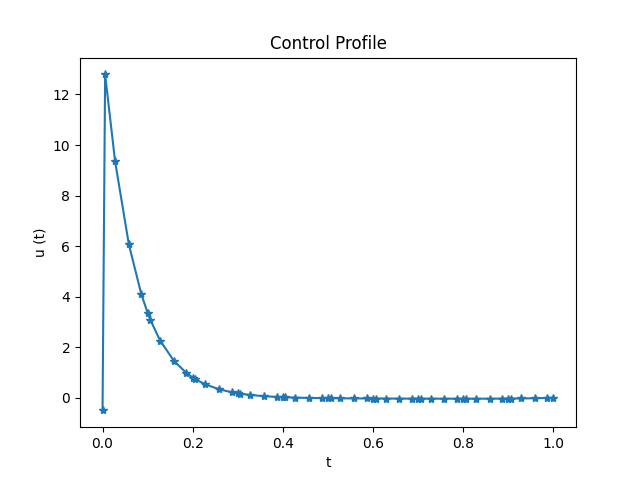
\includegraphics[width=5cm]{radau_control_profile.png}
  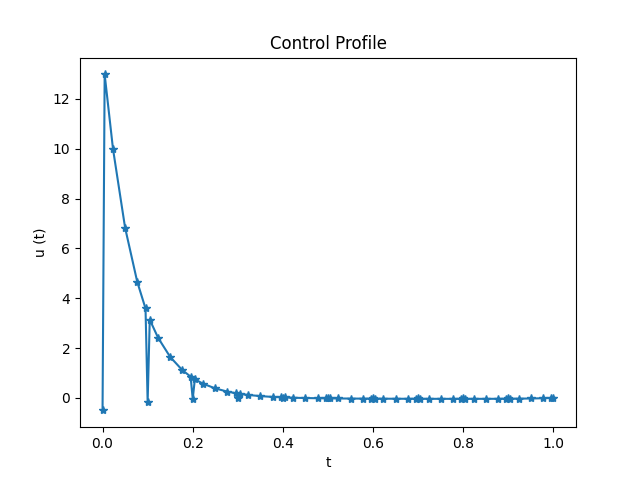
\includegraphics[width=5cm]{legendre_control_profile.png}
  \caption{Radau discretization, then legendre discretization}
\end{figure}

I suspect that the control variables are becoming arbitrary because they:
\begin{enumerate}
  \item Are free
  \item Have no effect on other variables
  \item Have no effect on the objective value
\end{enumerate}
How can I make this precise? First, I need to know which variables are my
inputs\ldots Just $u$ -- $x1$, $x2$, and $x3$ are states.
What is the path $u$ takes to influence the rest of the model, and why might
it be arbitrary here?

\[
u \rightarrow \frac{dx_1}{dt}, \frac{dx_2}{dt}, \frac{dx_3}{dt}
\rightarrow x_1, x_2, x_3 \text{ only at collocation points?}
\]

Things I'd like to check:
\begin{enumerate}
  \item What are all the variables ``influenced'' by $u$?
  \item Are there ``subsystems'' of model variables and equations that can
    be solved independently?
\end{enumerate}
What does Larry want us to answer?
\emph{Which variables can have arbitrary values?}
We suspect these are the control variables at non-collocation finite elements
points.
What is a sufficient condition for a variable to take an arbitrary value
during an optimization solve?
\begin{enumerate}
  \item It does not impact the value of the objective
  \item It is not part of a square subsystem\ldots, i.e. is not calculated
    by equality constraints.
\end{enumerate}
This is a bit tricky, as the variable value could be restricted by inequality
constraints.
How can I test if a variable influences the value of the objective?
If the variable ``influences the value'' of any of the variables in the
objective.
Given a matching and a DAG of variable calculation order, we can find the
variables necessary to calculate that one\ldots
This is more difficult in an optimization problem.

\end{document}
